\documentclass[10pt]{article}

% --- Language and Encoding ---
\usepackage[utf8]{inputenc}
\usepackage[T1]{fontenc}

% --- Fonts and Typography ---
\usepackage[scaled=0.92]{helvet}
\renewcommand{\familydefault}{\sfdefault}
\usepackage{microtype}

% --- Page Geometry ---
\usepackage[letterpaper, margin=0.6in, top=0.6in, bottom=0.6in]{geometry}

% --- Color Palette ---
\usepackage{xcolor}
\definecolor{primary}{HTML}{0B3C5D}
\definecolor{secondary}{HTML}{328CC1}
\definecolor{accent}{HTML}{D9B310}
\definecolor{darkneutral}{HTML}{1D2731}
\definecolor{lightneutral}{HTML}{F9F9F9}
\definecolor{bordergray}{HTML}{E2E8F0}

% --- Packages ---
\usepackage{amsmath, amssymb}
\usepackage{booktabs}
\usepackage{enumitem}
\usepackage{graphicx}
\usepackage{tikz}
\usetikzlibrary{positioning, calc, shapes.geometric, arrows.meta}
\usepackage[many]{tcolorbox}
\usepackage{hyperref}
\usepackage{fontawesome5}

\hypersetup{
    colorlinks=true,
    linkcolor=primary,
    filecolor=primary,      
    urlcolor=secondary,
    citecolor=primary,
}

% --- Custom Command for Section Headers in Abstract ---
\newcommand{\abstractsection}[1]{\vspace{0.12cm}\noindent\textbf{\color{primary}\fontsize{9}{11}\selectfont #1}\par\vspace{0.03cm}}

\begin{document}
\pagestyle{empty}

% --- Header Band ---
\noindent
\begin{tcolorbox}[
    colback=primary,
    colframe=primary,
    arc=4pt,
    left=10pt,
    right=10pt,
    top=5pt,
    bottom=5pt,
    boxrule=0pt
]
    \begin{minipage}[c]{0.7\textwidth}
        \textcolor{white}{\fontsize{9.5}{11.5}\sffamily\bfseries\scshape 12th Annual Apex Student Research Symposium (ASRS 2026)} \\
        \textcolor{accent}{\fontsize{8}{10}\sffamily\bfseries Track: Autonomous Systems \& Intelligent Robotics}
    \end{minipage}\hfill
    \begin{minipage}[c]{0.25\textwidth}
        \flushright
        \textcolor{white}{\fontsize{8}{10}\sffamily Abstract ID: \textbf{ASRS-2026-042}} \\
        \textcolor{white}{\fontsize{8}{10}\sffamily Format: \textbf{Oral Presentation}}
    \end{minipage}
\end{tcolorbox}

\vspace{0.2cm}

% --- Title Block ---
\noindent
\begin{tcolorbox}[
    colback=white,
    colframe=secondary,
    leftrule=4pt,
    rightrule=0pt,
    toprule=0pt,
    bottomrule=0pt,
    arc=0pt,
    outer arc=0pt,
    left=10pt,
    right=0pt,
    top=0pt,
    bottom=0pt,
    boxsep=0pt
]
    {\fontsize{15}{18}\sffamily\bfseries\color{primary} Autonomous Path Planning for Unmanned Aerial Vehicles in GPS-Denied Environments using SynapseNet}\\[0.12cm]
    
    {\fontsize{10}{12}\sffamily\bfseries Sarah L. Jenkins\textsuperscript{1,*}, Dr. Marcus Vance\textsuperscript{1}, and Prof. Elena Rostova\textsuperscript{2}}\\[0.08cm]
    
    {\fontsize{8}{10}\sffamily\color{darkneutral} 
    \textsuperscript{1}Department of Intelligent Systems, Vertex Institute of Technology, Apex City \\
    \textsuperscript{2}Center for Complex Systems, Meridian Research Laboratory, Nimbus District\\[0.05cm]
    \textsuperscript{*}Corresponding presenter: \href{mailto:s.jenkins@vertex.edu}{\texttt{\faEnvelope\ s.jenkins@vertex.edu}}
    }
\end{tcolorbox}

\vspace{0.2cm}
\noindent{\color{secondary}\rule{\textwidth}{1.2pt}}
\vspace{0.2cm}

% --- Main Content Columns ---
\noindent
\begin{minipage}[t]{0.63\textwidth}
    \fontsize{8.5}{11}\selectfont
    \abstractsection{Introduction \& Motivation}
    Autonomous navigation of unmanned aerial vehicles (UAVs) in GPS-denied environments is a critical challenge in search-and-rescue, structural inspection, and forest fire tracking. Traditional state-estimation and navigation pipelines suffer from cumulative drift when primary sensor feeds are degraded. While deep reinforcement learning (DRL) provides a promising alternative, existing architectures fail to capture long-term temporal dependencies and struggle to adjust to dynamic obstacle fields in real time. We address this limitation by proposing \textit{SynapseNet}, a novel spatio-temporal neural network designed specifically for real-time onboard path planning under severe sensor constraints.

    \abstractsection{Methodology}
    Our methodology comprises a hybrid deep network architecture integrated directly into the UAV flight controller. The model features:
    \begin{itemize}[leftmargin=*,noitemsep,topsep=1.5pt,parsep=0.5pt]
        \item \textbf{Spatial Attention Mechanism:} Focuses computational resources on critical obstacle boundaries detected via lightweight solid-state LiDAR.
        \item \textbf{Temporal Convolutional Layers:} Processes sequences of past states to predict trajectory drift and correct velocity vectors.
        \item \textbf{Kinematic Projection Layer:} A custom layer that projects neural network outputs onto the UAV's physical constraints, ensuring smooth, executable trajectories.
    \end{itemize}
    Training was performed in the high-fidelity \textit{Nimbus Sim} environment, using curriculum learning to transition from static environments to dynamic wind-shear fields.

    \abstractsection{Results \& Performance Analysis}
    The framework was evaluated across 500 randomized, cluttered scenarios and compared against standard industry baselines. As summarized in Table 1, SynapseNet achieved a navigation success rate of 94.2\%, outperforming the Apex baseline by 15.8\% while maintaining a computationally efficient footprint. The integration of temporal modeling yielded a 22.4\% reduction in trajectory drift compared to purely spatial models. Crucially, inference latency remained well below the 15-millisecond threshold required for closed-loop stability on low-power edge computers.

    \abstractsection{Conclusion \& Future Work}
    This work demonstrates the viability of attention-guided temporal architectures for robust, autonomous UAV operations without GPS dependencies. Future research will focus on the deployment of SynapseNet onto physical quadcopters for field validation within the Meridian forest reserves.
\end{minipage}
\hfill
\begin{minipage}[t]{0.33\textwidth}
    % Right Side Content: Table, TikZ diagram, Keywords
    
    \noindent
    \begin{tcolorbox}[
        colback=lightneutral,
        colframe=bordergray,
        arc=4pt,
        left=6pt,
        right=6pt,
        top=5pt,
        bottom=5pt,
        boxrule=1pt,
        fonttitle=\bfseries\sffamily\color{primary}\fontsize{8}{10}\selectfont,
        title=Performance Comparison,
        colbacktitle=lightneutral,
        attach title to upper,
        after title={\par\smallskip}
    ]
        \centering
        \fontsize{7}{9}\sffamily
        \begin{tabular}{lcc}
            \toprule
            \textbf{Algorithm} & \textbf{Success (\%)} & \textbf{Latency (ms)} \\
            \midrule
            Apex Base & 78.4 & \phantom{0}8.5 \\
            Vertex-Path & 82.1 & 15.2 \\
            \textbf{SynapseNet} & \textbf{94.2} & \textbf{11.4} \\
            \bottomrule
        \end{tabular}
        \par\vspace{0.08cm}
        {\fontsize{6.5}{8}\color{darkneutral}\textit{Table 1: Simulation benchmarks.}}
    \end{tcolorbox}
    
    \vspace{0.15cm}
    
    \noindent
    \begin{tcolorbox}[
        colback=lightneutral,
        colframe=bordergray,
        arc=4pt,
        left=6pt,
        right=6pt,
        top=5pt,
        bottom=5pt,
        boxrule=1pt,
        fonttitle=\bfseries\sffamily\color{primary}\fontsize{8}{10}\selectfont,
        title=Architecture Overview,
        colbacktitle=lightneutral,
        attach title to upper,
        after title={\par\smallskip}
    ]
        \centering
        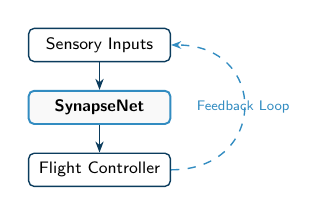
\begin{tikzpicture}[
            node distance=0.35cm,
            align=center,
            box/.style={rectangle, draw=primary, fill=white, rounded corners=2pt, minimum width=1.8cm, minimum height=0.42cm, line width=0.5pt},
            accentbox/.style={rectangle, draw=secondary, fill=lightneutral, rounded corners=2pt, minimum width=1.8cm, minimum height=0.42cm, line width=0.7pt}
        ]
            % Nodes
            \node[box] (sensor) {\fontsize{6.5}{8}\selectfont Sensory Inputs};
            \node[accentbox, below=of sensor] (net) {\fontsize{6.5}{8}\selectfont \textbf{SynapseNet}};
            \node[box, below=of net] (controller) {\fontsize{6.5}{8}\selectfont Flight Controller};
            
            % Arrows
            \draw[-{Stealth[scale=0.7]}, line width=0.6pt, primary] (sensor) -- (net);
            \draw[-{Stealth[scale=0.7]}, line width=0.6pt, primary] (net) -- (controller);
            
            % Feedback loop
            \draw[-{Stealth[scale=0.7]}, line width=0.5pt, secondary, dashed] (controller.east) to[out=0, in=0, looseness=2.0] (sensor.east);
            \node[right=0.2cm of net, anchor=west, text=secondary] {\fontsize{5.5}{7}\selectfont Feedback Loop};
        \end{tikzpicture}
        \par\vspace{0.08cm}
        {\fontsize{6.5}{8}\color{darkneutral}\textit{Figure 1: Navigation schematic.}}
    \end{tcolorbox}
    
    \vspace{0.15cm}
    
    \noindent
    \begin{tcolorbox}[
        colback=lightneutral,
        colframe=bordergray,
        arc=4pt,
        left=6pt,
        right=6pt,
        top=5pt,
        bottom=5pt,
        boxrule=1pt
    ]
        \fontsize{7.5}{9.5}\sffamily
        \textbf{\color{primary}Keywords:}\\
        Autonomous Flight, Spatio-Temporal Models, Spatial Attention, Path Planning, SynapseNet
    \end{tcolorbox}
\end{minipage}

\vspace{0.25cm}

% --- Funding & Acknowledgements Section ---
\noindent
\begin{tcolorbox}[
    colback=lightneutral,
    colframe=secondary,
    arc=4pt,
    boxrule=0.5pt,
    left=10pt,
    right=10pt,
    top=5pt,
    bottom=5pt
]
    \fontsize{8}{10}\sffamily
    \textbf{\color{primary}Acknowledgements \& Funding}\\
    This research was supported in part by the Apex Science Foundation under Grant No. ASF-2025-089. Computational resources were generously provided by the Nimbus Cloud Infrastructure Initiative. The authors thank the members of the Vertex Robotics Lab for their valuable feedback and technical support during simulation setup.
\end{tcolorbox}

\end{document}
